\let\negmedspace\undefined
\let\negthickspace\undefined
\documentclass[journal,12pt,twocolumn]{IEEEtran}
\usepackage{cite}
\usepackage{amsmath,amssymb,amsfonts,amsthm}
\usepackage{algorithmic}
\usepackage{graphicx}
\usepackage{textcomp}
\usepackage{xcolor}
\usepackage{txfonts}
\usepackage{listings}
\usepackage{enumitem}
\usepackage{mathtools}
\usepackage{gensymb}
\usepackage[breaklinks=true]{hyperref}
\usepackage{tkz-euclide} % loads  TikZ and tkz-base
\usepackage{listings}
\usepackage{geometry}

\geometry{margin=1in}

% correct bad hyphenation here
\hyphenation{op-tical net-works semi-conduc-tor}
\def\inputGnumericTable{}       

\lstset{
%language=C,
frame=single, 
breaklines=true,
columns=fullflexible
}

\begin{document}

\vspace{3cm}

\title{Randomized Playlist Generation in Python \\ AI1110}
\author{Edward Nathan Varghese \\ CS22BTECH11020}


\maketitle

\section{Introduction}
This report summarizes and analyses my implementation of a randomized playlist generator in Python using Numpy, Tkinter, Pygame and Playsound modules.

\section{Code Explanation}
\begin{itemize}
  \item The beginning of the code has import statements for the required modules.
  \item \texttt{Construct()} is the randomizer and list populator. It uses the uniform distribution and returns a float from 0 to 20 which is passed to the \texttt{ceil()} function to return an integer between 1 and 20. It then populates a list \texttt{songnums} with a random sequence of numbers from 1 - 20.
  \item A class \texttt{Playlist} is created and the Tkinter window and widgets are initialized along with the functions needed for the code  such as \texttt{playsong()}, \texttt{autoplay()} and \texttt{pause\_resume()}.
  \item The buttons on the main window call their respective functions which are breifly descibed below.
  \item \texttt{playsong()} plays the next song in \texttt{songnums} using \texttt{pygame.mixer.music.play()}.
  \item \texttt{autoplay()} ensures continuity of the playlist and makes sure the next song plays after the current one has ended.
  \item \texttt{pause\_resume()} controls the state of the songs, whether they are being played or not. This is done using the \texttt{pygame.mixer.music.pause()} and \texttt{pygame.mixer.music.unpause()} statements.
  \item The GUI layout is organized using the grid system, and the buttons are placed in different rows and columns within the root window.
  \item Finally, we create the root window and an object of \texttt{Playlist} called \texttt{MyPlaylist} is created and the main event loop is started using \texttt{root.mainloop()}.
\end{itemize}

\section{Output}
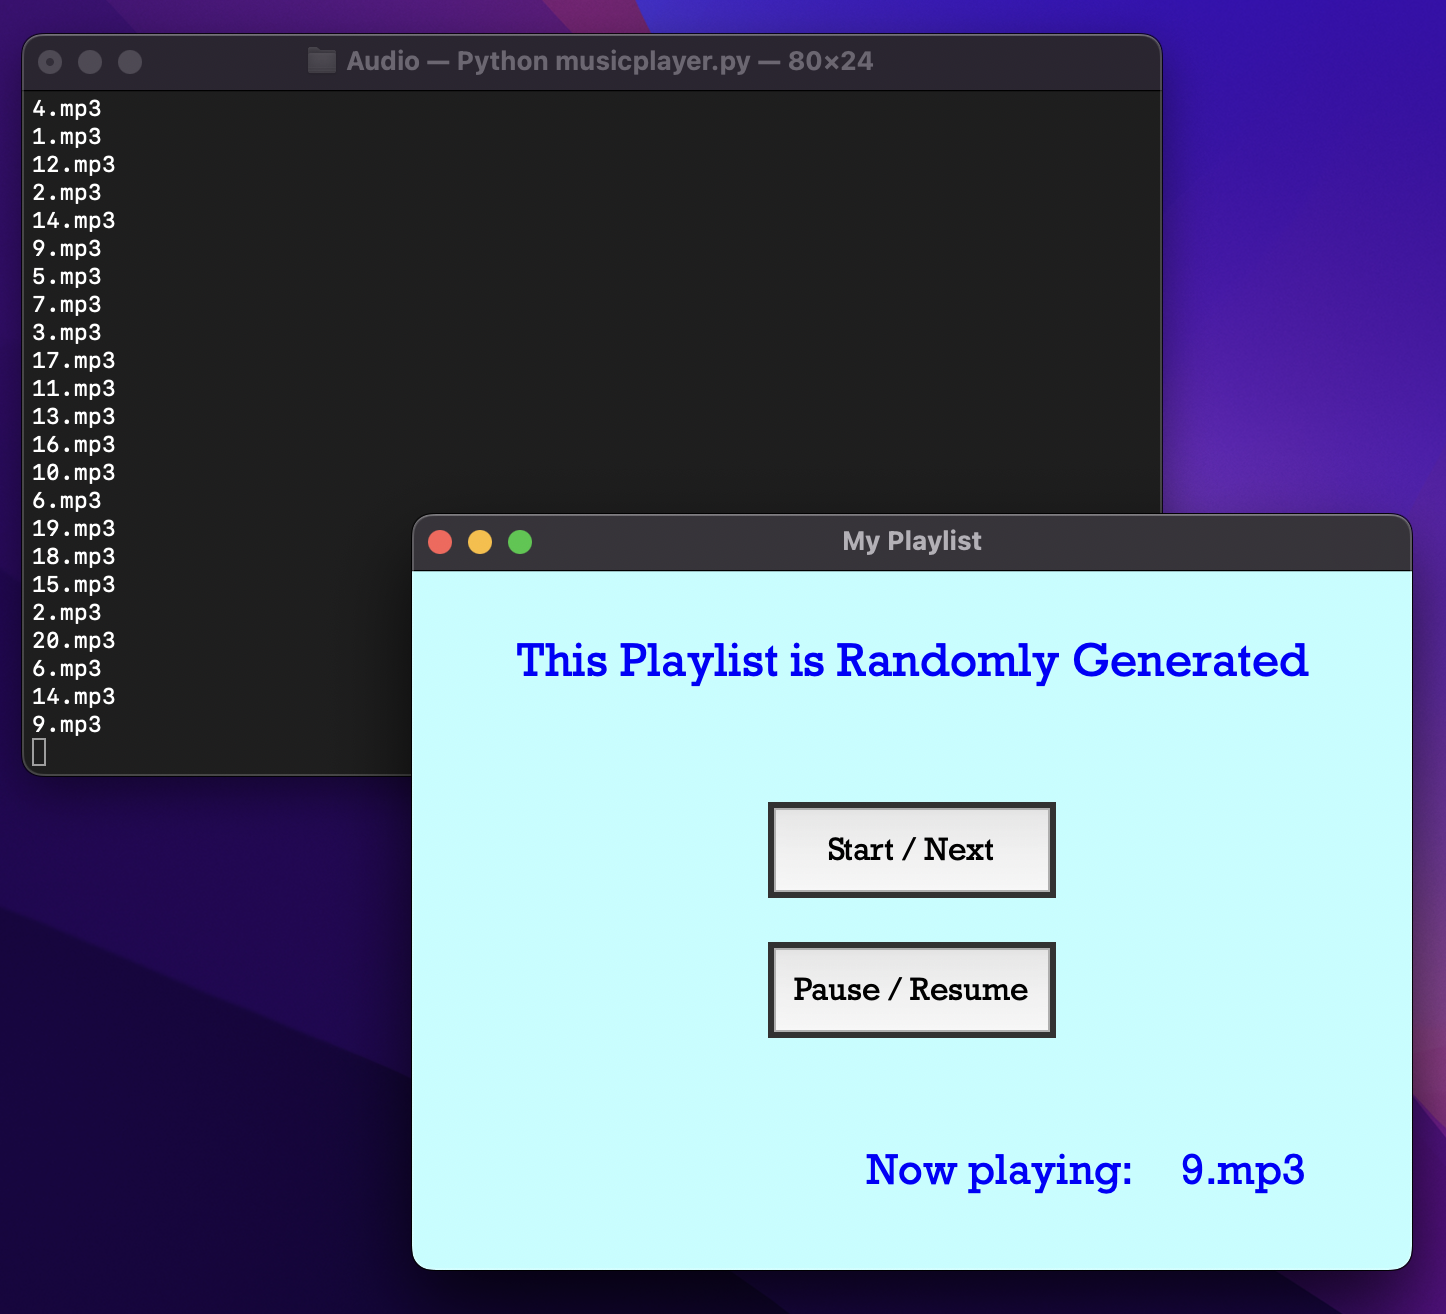
\includegraphics[scale=0.36]{images/Output.png}

\section{Conclusion}
This code is a basic implementation of a Randomised Music Playlist in Python using Numpy, Tkinter, Playsound and Pygame modules.
\end{document}
